\section{Auswertung}
\subsection{Bestimmung der Aktivität}
Die Aktivität der Probe wird mithilfe des Zerfallsgesetzes 
\begin{equation}
    A = A_0 \cdot e^{-\frac{\ln{2}}{\tau}t}
\end{equation}

\begin{center}
    \tiny{($A_0 $ $\hat{=}$ Ursprüngliche Aktivität der Probe, $\tau$ $\hat{=}$ Halbwertszeit der Probe, $t$ $\hat{=}$ vergangene Zeit )}
\end{center}
bestimmt. 
Mit der in Oktober 1994 gemessenden Aktiviät $A_0 = \SI{330}{\kilo\becquerel}$, der Halbwertszeit von $\tau = \SI{432.6(6)}{\second}$ von $^{241}{Am}$ und der seit Oktober 1994 vergangenden Zeit $t = \SI{7,897(13)e8}{\second}$ ergibt sich für die Aktivität
\begin{equation}
    A_\text{theo} = \SI{3.170(10)e5}{\kilo\becquerel} .
\end{equation}
Um die Aktivität experimentell zu bestimmen, wird zunächst eine Nullmessung im Vakuum von $\SI{87,7}{\milli \bar}$ durchgeführt. Dabei wurden innerhalb von $t=\SI{68}{\second}$ $N=1064(32)$ Ereignisse registriert, wobei sich die Unsicherheit $\sigma_N$ aus der Poissonverteilung ergibt. 
Mit diesen Werten folgt für die Aktivität
\begin{equation}
    \frac{\Omega}{4 \pi } \cdot  A_\text{exp} = A_\text{exp0} = \frac{N}{t} = \SI{15.64(48)}{\kilo\becquerel} ,
\end{equation}
wobei die Unsicherheit $\sigma_{ A_\text{exp}} = \frac{\sigma_N}{t}$ aus der Gaußschen Fehlerfortpflanzung folgt. 
Dies ist jedoch lediglich die Aktivität, die im Raumwinkelelement $\frac{\Omega}{4 \pi}$ erfasst wurde. Wenn davon ausgegangen wird, dass die auf dem Detektor aktive Fläche Teil einer Kugel mit $r = \SI{101}{\milli \meter}$ entspricht - wobei $r$ den Abstand zwischen Detektor und Quelle darstellt. 
Das Verhältnis der Flächen wird aufgrund der beiden aktiven  $\SI{2}{\milli \meter}$ Schlitzblenden auf 
\begin{equation}
    \frac{\Omega}{4 \pi } = \frac{2 \cdot 4 \si{\milli \meter}^2}{101^2 \si{\milli \meter}^2 \cdot 4\pi } = 3,12 \cdot 10^{-5}
\end{equation}
geschätzt.
Somit folgt für die Aktivität
\begin{equation}
    A_\text{exp} = \SI{501(15)}{\kilo\becquerel} .
\end{equation}
Auch hier folgt die Unsicherheit aus der Gaußschen Fehlerfortpflanzung: 
\begin{equation}
    \sigma_\text{Aexp} =  \frac {\sigma_\text{Aexp}}{\frac{\Omega}{4 \pi }} 
\end{equation} 

\subsection{Bestimmung der Foliendicke mittels Energieverlustmessung}
Die Foliendichte wird mithilfe eines Oszilloskops bestimmt. Mit diesem werden die Spannungen $U$ einzlener Impulse bei verschiedenen Drücken $p$ aufgenommen. Diese Messung wird einmal mit und einmal ohne eingebauter Goldfolie durchgeführt. Die Messwerte befinden sich in den Tabellen \ref{tab:mit} und \ref{tab:ohne2}.
\begin{table}[H]
   \centering
   \caption{Gemessene Spannungen $U$ und Drücke $p$ mit Goldfolie.}
   \label{tab:mit}
   \begin{tabular} { c c }
 \toprule
 {$\text{Druck}\:/\: \mathrm{mbar}$} & {$\text{Pulshöhe}\:/\: \mathrm{V}$} \\ 
    \midrule
    91,6 & 8,64 \\
    105 & 7,60 \\
    110 & 6,88 \\
    130 & 6,24 \\
    140 & 5,68 \\
    150 & 5,28 \\
    170 & 4,56 \\
    180 & 4,56 \\
    200 & 5,52 \\
    230 & 5,52 \\
    300 & 3,92 \\
    400 & 3,92 \\
    500 & 3,92 \\
    \bottomrule
  \end{tabular}
\end{table}

\begin{table}[H]
   \centering
   \caption{Gemessene Spannungen $U$ und Drücke $p$ ohne Goldfolie.}
   \label{tab:ohne2}
   \begin{tabular} { c c }
 \toprule
 {$\text{Druck}\:/\: \mathrm{mbar}$} & {$\text{Pulshöhe}\:/\: \mathrm{V}$} \\ 
    \midrule
    80 & 11,40 \\
    100 & 11,40 \\
    110 & 11,60 \\
    120 & 11,30 \\
    140 & 9,12 \\
    150 & 7,90 \\
    160 & 8,60 \\
    180 & 7,04 \\
    190 & 6,08 \\
    200 & 5,36 \\
    220 & 3,04 \\
    240 & 2,80 \\
    260 & 3,30 \\
    280 & 4,40 \\
    \bottomrule
  \end{tabular}
\end{table}

Um von den in den Tabellen \ref{tab:mit} und \ref{tab:ohne2} auf die Foliendicke schließen zu können, wird zunächst eine Ausgleichsrechnung der Form
\begin{equation}
    U = a \cdot p + b 
\end{equation}
durchgeführt.
Daraus ergeben sich die Parameter
\begin{align*}
    a_\text{ohne} &= (-0,895 \pm 240) \cdot 10^{-2} \si{\volt\per\milli\per\bar} \\
    b_\text{ohne} &= (7,421 \pm 0,575) \si{\milli\bar} \\
    a_\text{mit} &=  (-5,048 \pm 0,517) \cdot 10^{-2} \si{\volt\per\milli\per\bar} \\
    b_\text{mit} &=  (16,144 \pm 0,948) \si{{\milli\bar}} . \\
\end{align*}
Dabei gehören die Parameter mit dem Index $\texttt{ohne}$ zu Versuchsreihe ohne eingesetzter Goldfolie, während die Parameter mit dem Index $\texttt{mit}$ zu Versuchsreihe mit eingesetzter Goldfolie gehören. Die dazugehörigen Graphen befinden sich in Abbildung \ref{fig:geraden}.
\begin{figure}[H]
    \centering
    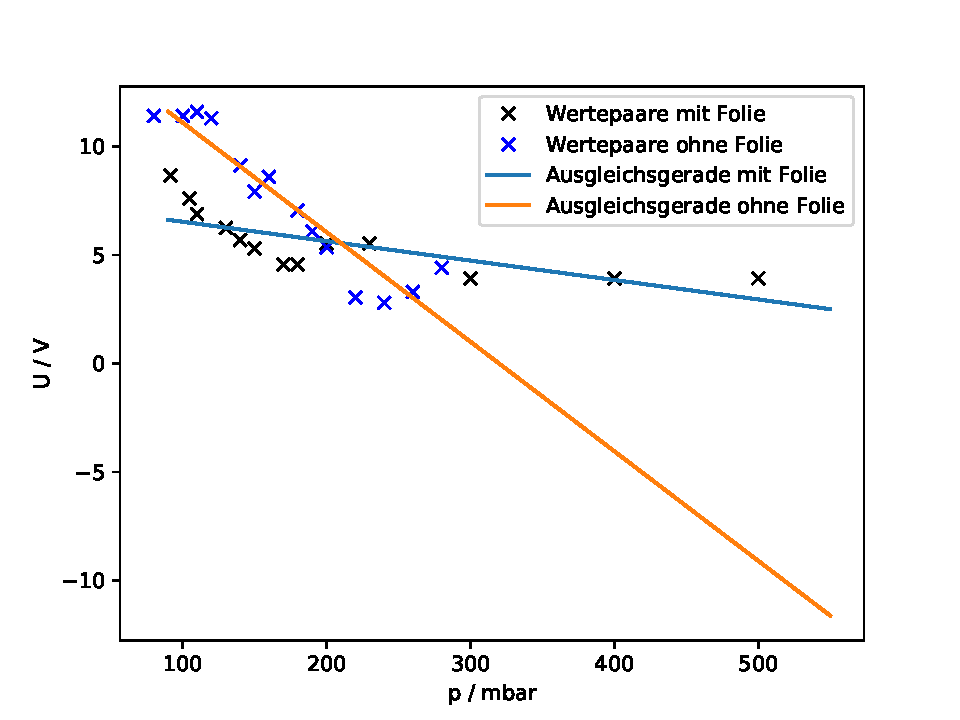
\includegraphics[width=0.8\textwidth]{data/plots/gerade.pdf}
    \caption{Spannung $U$ aufgetragen gegen Druck $p$, mit und ohne Folie.}
    \label{fig:geraden}
\end{figure}

Um nun mithilfe der Bethe-Bloch Formel \eqref{eqn:bethebloch} auf den Energieverlust schließen zu können, wird zunächst ein Umrechnungsfaktor $\kappa$ von Spannung und Energie bestimmt. Die Energie der $\alpha$-Teilchen ist aus der Theorie bekannt und gegeben mit $E_\alpha = \SI{5,486}{\mega \electronvolt}$.
Damit folgt 
\begin{equation}
    \kappa = \frac{E_\alpha}{b_\text{ohne}} = (0,340 \pm 0,020) \si{\mega \electronvolt \per \volt}, 
\end{equation}
wobei die Unsicherheit $\sigma_\kappa$ aus der Gaußschen Fehlerfortpflanzung $\sigma_\kappa = \frac{E_\alpha}{b_\text{ohne}}\sigma_{b_\text{ohne}}$ folgt. \\
Der Energieverlust beträgt somit
\begin{equation}
    \Delta E = \kappa \cdot (b_\text{ohne}-b_\text{mit}) = \SI{2,96(25)}{\mega \electronvolt}
\end{equation} 
deren Unsicherheit $\sigma_E$ aus der Gaußschen Fehlerfortpflanzung
\begin{align*}
    \sigma_E &= \sqrt{(b_\text{ohne}-b_\text{mit})^2\sigma_\kappa^2+\kappa^2\left(\sigma_{b_\text{ohne}}^2+\sigma_{b_\text{mit}}^2\right)}\text{.}
\end{align*}
folgt. \\
Zusammen mit Formel \eqref{eqn:bethebloch} und 
\begin{equation*}
    v^2=\frac{2\bar{E}}{m_\text{\alpha}}=\frac{E_{\alpha}}{m_\text{\alpha}}\left(1+\frac{b_\text{mit}}{b_\text{ohne}}\right)
\end{equation*}
folgt für die Dicke $d$ der Folie
\begin{equation*}
    d = \SI{6,5(5)}{\micro \meter}
\end{equation*} 

\subsection{Untersuchung des differentiellen Wirkungsquerschnittes einer dünnen Goldfolie} \label{chap:dsdO}
Im folgenden wird der differentielle Wirkungsquerschnitt einer $\SI{2}{\micro \meter}$ dünnen Goldfolie untersucht. Dieser lässt sich experimentell mit der Formel \cite{Kroeninger}
\begin{equation}
    \left(\frac{\symup{d}\sigma}{\symup{d}\Omega}\right)_\text{exp} = \frac{I}{A \cdot n \cdot d \cdot \Omega}
    \label{eqn:dsdO_exp}
\end{equation}
\begin{center}
    \tiny{($n$ $\hat=$ Teilchendichte, $d$ $\hat=$ Teilchendichte, $\Omega = \frac{\pi r^2}{R^2} \hat{=}$ Vom Detektor abgedeckter Raumwinkel )}
\end{center}
bestimmen. \\
Mit der bereits bestimmten Aktivität $\SI{15.64(48)}{\kilo\becquerel}$ ergeben sich die Werte in Tabelle \ref{tab:diffWQ}. \\
Die gemessenen und theoretischen Werte sind zusätzlich in Abbildung \ref{fig:ruther} gegenübergestellt.
\begin{table}[H] 
   \centering 
   \caption{Die gemessenen Größen und die dazu ausgerechneten differentiellen Wirkungsquerschnitte} 
   \label{tab:diffWQ} 
   \begin{tabular} { c c c c c } 
 \toprule 
 {$Theta\:/\: \mathrm{°}$} & {$N$} & {$t\:/\: \mathrm{s}$} & {$\left(\frac{\mathrm{d}\sigma}{\mathrm{d}\Omega}\right)_\text{exp}/10^{-24}\si{\meter^2}$} & {$\left(\frac{\mathrm{d}\sigma}{\mathrm{d}\Omega}\right)_\text{theo}/10^{-24}\si{\meter^2}$} \\ 
    \midrule 
    -0,1 & 1047+/-32 & 116,0 & $(1,046+/-0,0) \cdot 10^{-22}$ & $(1,853)\cdot 10^{-16}$ \\ 
    -0,2 & 1240+/-35 & 140,0 & $(1,026+/-0,0) \cdot 10^{-22}$ & $(1,158)\cdot 10^{-17}$ \\ 
    -0,3 & 1040+/-32 & 106,0 & $(1,137+/-0,0) \cdot 10^{-22}$ & $(2,288)\cdot 10^{-18}$ \\ 
    -0,4 & 1050+/-32 & 122,0 & $(9,97+/-0,31) \cdot 10^{-23}$ & $(7,240)\cdot 10^{-19}$ \\ 
    -0,5 & 1060+/-33 & 110,0 & $(1,116+/-0,0) \cdot 10^{-22}$ & $(2,965)\cdot 10^{-19}$ \\ 
    -0,6 & 1030+/-32 & 111,0 & $(1,075+/-0,0) \cdot 10^{-22}$ & $(1,430)\cdot 10^{-19}$ \\ 
    -0,7 & 1050+/-32 & 119,0 & $(1,022+/-0,0) \cdot 10^{-22}$ & $(7,719)\cdot 10^{-20}$ \\ 
    -0,8 & 1090+/-33 & 119,0 & $(1,061+/-0,0) \cdot 10^{-22}$ & $(4,525)\cdot 10^{-20}$ \\ 
    -0,9 & 1021+/-32 & 125,0 & $(9,46+/-0,30) \cdot 10^{-23}$ & $(2,825)\cdot 10^{-20}$ \\ 
    -1,0 & 1226+/-35 & 132,0 & $(1,076+/-0,0) \cdot 10^{-22}$ & $(1,853)\cdot 10^{-20}$ \\ 
    -1,2 & 1038+/-32 & 133,0 & $(9,04+/-0,28) \cdot 10^{-23}$ & $(8,939)\cdot 10^{-21}$ \\ 
    -1,4 & 1035+/-32 & 113,0 & $(1,061+/-0,0) \cdot 10^{-22}$ & $(4,825)\cdot 10^{-21}$ \\ 
    -1,6 & 1060+/-33 & 131,0 & $(9,37+/-0,29) \cdot 10^{-23}$ & $(2,828)\cdot 10^{-21}$ \\ 
    -1,8 & 1000+/-32 & 130,0 & $(8,91+/-0,28) \cdot 10^{-23}$ & $(1,765)\cdot 10^{-21}$ \\ 
    -2,0 & 1140+/-34 & 93,0  & $(1,42+/-0,04) \cdot 10^{-22}$ & $(1,158)\cdot 10^{-21}$ \\ 
    -2,5 & 1028+/-32 & 143,0 & $(8,33+/-0,26) \cdot 10^{-23}$ & $(4,746)\cdot 10^{-22}$ \\ 
    -3,0 & 1270+/-40 & 206,0 & $(7,14+/-0,20) \cdot 10^{-23}$ & $(2,289)\cdot 10^{-22}$ \\ 
    \bottomrule 
  \end{tabular}
\end{table}

\begin{figure}
    \centering
    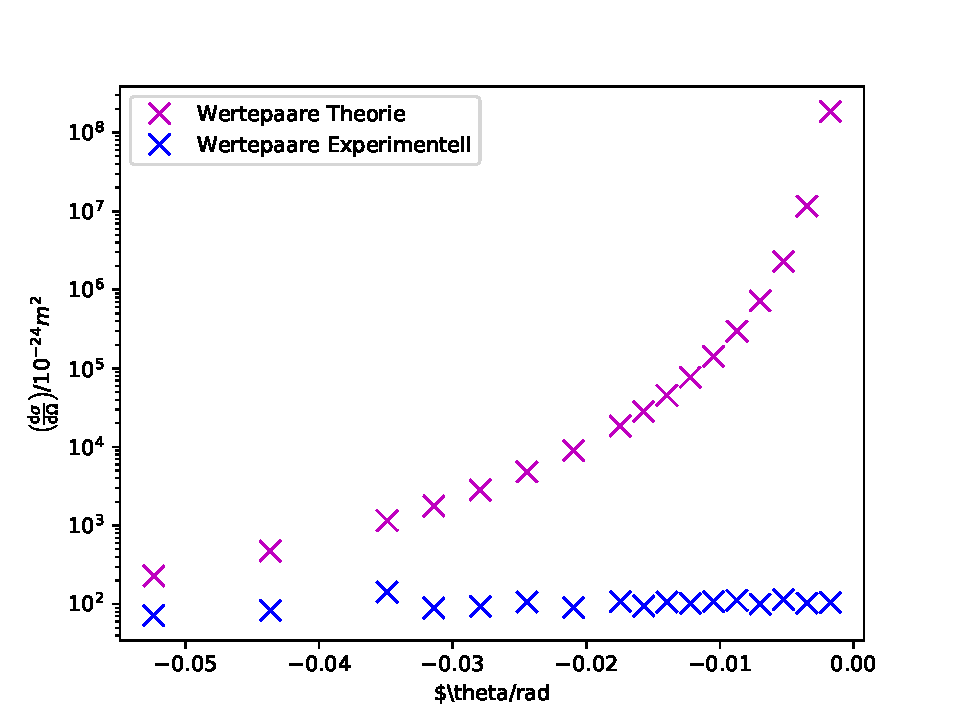
\includegraphics[width=0.8\textwidth]{data/plots/Rutherford.pdf}
    \caption{Differentieller und theoretischer Wirkungsquerschnitt $\frac{\symup{d}\sigma}{\symup{d}\Omega}$ gegen den Winkel $\theta$ aufgetragen. Die Unsicherheit wurde mit dem Faktor 100 multipliziert, damit dieser noch sichtbar ist.}
    \label{fig:ruther}
\end{figure}

\subsection{Untersuchung des Einflusses der Mehrfachstreuung}
Um zu untersuchen, ob bei dickeren Folien Mehrfachstreuung auftritt, wird die Intensität $I$ für zwei verschieden dicke Goldfolien an einem festen Winkel $\theta$ gemessen. \\
Mit den in Tabelle \ref{tab:foliendicke} gemessenden Werten ergeben sich die folgenden Wirkungsquerschnitte
\begin{align*}
    \left(\frac{\symup{d}\sigma}{\symup{d}\Omega}\right)_\text{\SI{2}{\micro \meter}} &= \SI{1,076(31)e-22}{\meter}^2 \\
    \left(\frac{\symup{d}\sigma}{\symup{d}\Omega}\right)_\text{\SI{4}{\micro \meter}} &= \SI{5,0(10)e-25}{\meter}^2
\end{align*} 
\begin{table}[H]
   \centering
   \caption{Dicke der Goldfolien in \si{\micro \meter}, Anzahl der gemessenen Ereignisse $N$ und die gemessene Zeit $t$}
   \label{tab:foliendicke}
   \begin{tabular} { c c c }
 \toprule
 {Foliendicke\:/\: $\si{\micro \meter}$} & \text{Ereignisse} & {Zeit\:/\: $\mathrm{s}$} \\ 
    \midrule
    2 & 1226 & 132 \\
    4 & 26 & 300 \\
    \bottomrule
  \end{tabular}
\end{table}


\subsection{Z-Abhängigkeit des Wirkungsquerschnittes}
Um die Z-Abhängigkeit der Intensität zu bestimmen, wird die Intensität einer Streung an Gold, Aluminium und Bismuth bei gleichem Winkel $\theta$ bestimmt. Wie bereits in Kapitel \ref{chap:dsdO} wird hier der der differentielle Wirkungsquerschnitt $(\frac{\symup{d}\sigma}{\symup{d}\Omega}$ mithilfe von Gleichung \ref{eqn:dsdO_exp} bestimmt. 
Die dazu benötigten Teilchendichten befinden sich in Tabelle \ref{tab:zWerte}.
\begin{table}
\centering 
   \caption{Sowohl Kernladungszahl $Z$, Dicke der Folie $d$, als auch die Teilchendichte $n$ für Aluminium, Gold und Bismuth \cite{Elemente16}.} 
   \label{tab:zWerte}
    \begin{tabular}{lS[table-format=2.0]S[table-format=1.0]S[table-format=1.1]}
        \toprule
        {Element} & {$Z$} & {$d/\si{\micro\metre}$} & {$n/10^{28}\si{\metre^{-3}}$} \\
        \midrule
        {Aluminium} & 78 & 3 & 6.6  \\
        {Gold} & 79 & 2 & 5.9  \\
        {Bismut} & 83 & 1 & 2.9  \\
        \bottomrule
    \end{tabular}
\end{table}
Die aus diesen Daten bestimmten differentiellen Wirkungsquerschnitte werden daraufhin mit den mithilfe von Gleichung \eqref{eqn:bethebloch} berechneten theoretischen differentiellen Wirkungsquerschnitte berechnet.
Die Ergebnisse befinden sich in Tabelle \ref{tab:zWerte2} und sind nocheinmal grafisch in Abbildung \ref{fig:zWerte2} dargestellt.  
\begin{table}[H] 
   \centering 
   \caption{name} 
   \label{tab:name} 
   \begin{tabular} { c c c c c c c c } 
 \toprule 
 {$Material\:/\: \mathrm{-}$}  & {$Dicke\:/\: \mathrm{mu_meter}$} & {$Ereignisse\:/\: \mathrm{-}$} & {$Zeit\:/\: \mathrm{s}$} & {$Grad\:/\: \mathrm{°}$} & {$\left(\frac{\mathrm{d}\sigma}{\mathrm{d}\Omega}\right)_\text{exp}/10^{-23}\si{\meter^2}$} & {$\left(\frac{\mathrm{d}\sigma}{\mathrm{d}\Omega}\right)_\text{theo}/10^{-23}\si{\meter^2}$}\\ 
    \midrule 
    Aluminium & 3 & 523 & 300 & 4,2 & 6,41 & 3,45 \\ 
    Bismut & 2 & 551 & 300 & 4,2 & 1,06 & 5,96  \\ 
    Gold & 4 & 3515 & 300 & 4,2  & 6,91 & 6,58 \\ 
    \bottomrule 
  \end{tabular}
\end{table}
\begin{figure}
    \centering
    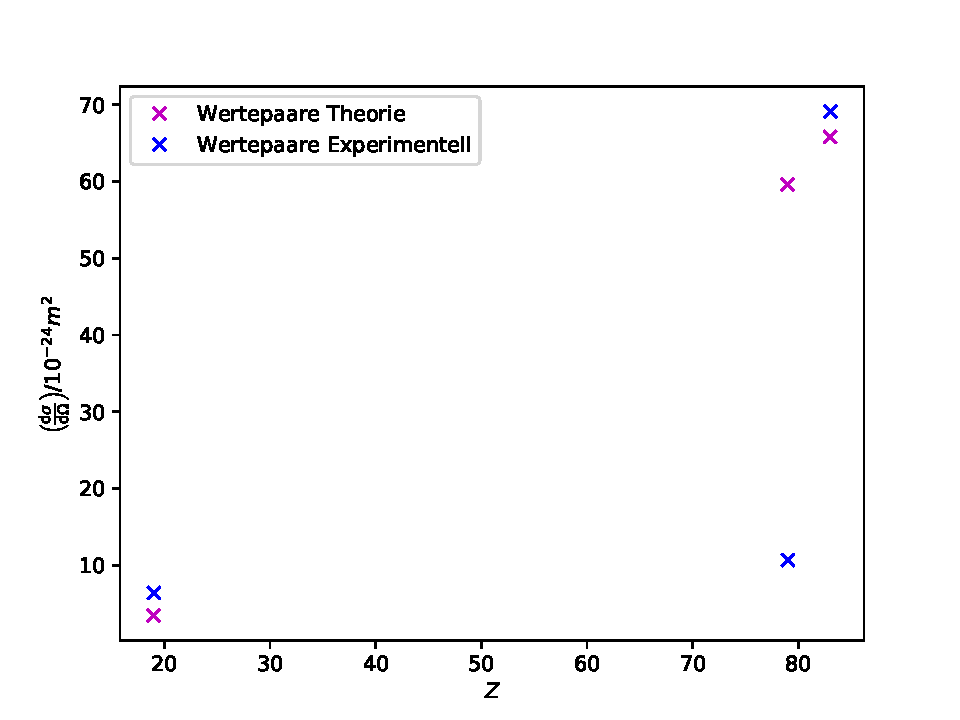
\includegraphics[width = 0.8\textwidth]{data/plots/atomic_number.pdf}
    \caption{Grafische Darstellung der differentiellen Wirkungsquerschnitte bei festem Winkel $theta$ und verschiedenen Ordnungszahlen $Z$.}
    \label{fig:zWerte2}
\end{figure}